\section{Tame knots}

It turns out that the simplest definition that capture the intuitive meaning if knot,
uses the closed polygonal lines.
An attempt to define knots as simple closed curves leads to a pathological examples as the one show on the diagram --- these are so called wild knots.

\begin{figure}[h]
\vskip-0mm
\centering
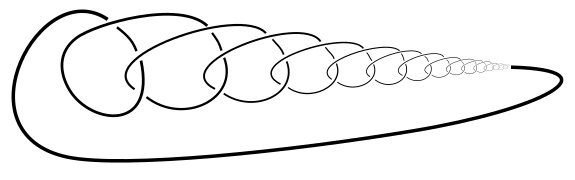
\includegraphics[scale=.6]{pics/Wild_knot}
\vskip0mm
\end{figure}

We define a \emph{knot} (more precicely \emph{tame knot}) to be a simple closed polygonal line in Euclidean space~$\RR^3$.

The notation $\triangle abc$ is used for triangle $abc$; that is a polygonal line with three edges and vertexes $a$, $b$ and $c$.
Let us denote by $\solidtriangle abc$ the convex hull of the points $a$, $b$ and $c$; $\solidtriangle abc$ is the solid triangle with the vertexes $a$, $b$ and $c$.
The points $a$, $b$ and $c$ are assumed to be distinct, but they might lie on one line;
that is for us a degenerate triangle is a triangle.

We understand a \emph{elementary deformation} of a knot to be the generation of a new knot from the original one by means of the
following two operations:

Assume $[pq]$ is an edge of the knot and $x$
is a point such that the solid triangle $\solidtriangle pqx$  has no common points with the knot except for the edge $[pq]$.
Then we can replace the edge $[pq]$ in the knot by two adjacent edges $[px]$ and $[xq]$.

We can also perform the inverse operation.
That is, if for two adjacent edges $[px]$ and $[xq]$ of a knot the triangle
$\solidtriangle pqx$ has no common points with the knot except for the points on the edges $[px]$ and $[xq]$,
then we can replace two adjacent edges $[px]$ and $[xq]$ by one edge $[pq]$.

Polygons that arise from one another by a finite sequence of
elementary deformations are called \emph{isotopic}.

A knot that is not isotopic to a triangle is called nontrivial.




